\section{Desain dan Implementasi}

Tugas ini dilakukan sesuai dengan desain sistem berikut beserta implementasinya. Desain sistem adalah konsep dari pembuatan dan perancangan infrastruktur dan kemudian diwujudkan dalam bentuk alur yang harus dikerjakan


\subsection{Deskripsi sistem}
Pada tugas ini kita akan melakukan analisis data dan membangun model regresi linier untuk memprediksi jumlah penonton video Youtube berdasarkan metadata yang tersedia. Proses ini melibatkan beberapa langkah, mulai dari eksplorasi data hingga evaluasi model. Desain sistem ini mencakup langkah-langkah yang akan dijabarkan dalam Gambar berikut.

\begin{figure}[ht]
    \centering
    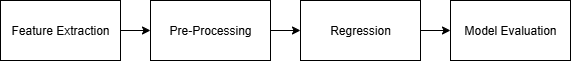
\includegraphics[width=0.8\textwidth]{gambar/metodologi.png}
    \caption{Blok Diagram Sistem}
    \label{fig:desain_sistem}
\end{figure}

\subsection{Feature Extraction}
Feature extraction adalah proses penting dalam machine learning yang bertujuan untuk mengidentifikasi dan memilih fitur-fitur yang relevan dari data yang tersedia. Dalam konteks tugas ini, kita akan melakukan feature extraction pada metadata video Youtube untuk mendapatkan fitur-fitur yang akan digunakan dalam model regresi linier.

\subsubsection{Deskripsi Dataset}
Dataset yang digunakan dalam tugas ini adalah dataset dalam format .xslx yang berisi metadata dari video Youtube. Dataset ini mencakup berbagai informasi seperti judul, deskripsi, tag, kategori, dan statistik penonton. Setiap baris dalam dataset mewakili satu video, dan kolom-kolomnya berisi fitur-fitur yang relevan untuk analisis. 
\newpage